\documentclass[conference,a4paper]{IEEEtran}
\IEEEoverridecommandlockouts

% ---------------------------------------------------------------- Paketler
\usepackage[utf8]{inputenc}
\usepackage[T1]{fontenc}
\usepackage[turkish]{babel}
\usepackage{lmodern}
\usepackage{amsmath,amssymb}
\usepackage{graphicx}
\usepackage{xcolor}
\usepackage{booktabs}
\usepackage{multirow}
\usepackage{array}
\usepackage{algorithm}
\usepackage{algpseudocode}
\usepackage{tikz}
\usetikzlibrary{babel,shapes.geometric,arrows.meta,positioning,fit,calc}
\usepackage{pgfplots}
\pgfplotsset{compat=1.17}
\usepackage{cite}
\usepackage{url}
\usepackage[hidelinks]{hyperref}

% ---------------------------------------------------------------- Türkçe ayarlar
\renewcommand{\IEEEkeywordsname}{Anahtar Kelimeler}
\floatname{algorithm}{Algoritma}
\renewcommand{\algorithmicrequire}{\textbf{Girdi:}}
\renewcommand{\algorithmicensure}{\textbf{Çıktı:}}
\renewcommand{\algorithmicif}{\textbf{eğer}}
\renewcommand{\algorithmicthen}{\textbf{ise}}
\renewcommand{\algorithmicelse}{\textbf{değilse}}
\renewcommand{\algorithmicwhile}{\textbf{iken}}
\renewcommand{\algorithmicfor}{\textbf{her}}
\renewcommand{\algorithmicdo}{\textbf{yap}}
\renewcommand{\algorithmicend}{\textbf{bitir}}
\renewcommand{\algorithmicreturn}{\textbf{döndür}}
\renewcommand{\algorithmicfunction}{\textbf{fonksiyon}}
\renewcommand{\algorithmicprocedure}{\textbf{yordam}}
\algrenewtext{EndWhile}{\textbf{döngü sonu}}
\algrenewtext{EndFor}{\textbf{döngü sonu}}
\algrenewtext{EndIf}{\textbf{koşul sonu}}
\algrenewtext{EndFunction}{\textbf{fonksiyon sonu}}
\algrenewtext{EndProcedure}{\textbf{yordam sonu}}

\newcommand{\kod}[1]{\texttt{#1}}

% ---------------------------------------------------------------- Ekran görüntüsü renkleri
% (Windows konsolunun varsayılan "Campbell" renk şeması)
\definecolor{tblack}{RGB}{12,12,12}
\definecolor{tdefault}{RGB}{204,204,204}
\definecolor{tgray}{RGB}{118,118,118}
\definecolor{tyellow}{RGB}{249,241,165}
\definecolor{tcyan}{RGB}{97,214,214}
\definecolor{tblue}{RGB}{0,55,218}
\definecolor{tcyanbg}{RGB}{58,150,221}
\definecolor{tlightgray}{RGB}{204,204,204}
\definecolor{tdarkgray}{RGB}{90,90,90}
\definecolor{tyellowbg}{RGB}{249,241,165}
\definecolor{tbrightblue}{RGB}{59,120,255}
\newcommand{\sstrut}{\rule[-0.32em]{0pt}{1.37em}}
\newcommand{\scell}[3]{{\setlength{\fboxsep}{0pt}\colorbox{#1}{\sstrut\textcolor{#2}{#3}}}}
\newcommand{\scellcur}[3]{\scell{#1}{#2}{#3}\llap{\textcolor{white}{\rule[-0.32em]{0.12em}{1.37em}}\hspace{0.405em}}}
\newcommand{\ekran}[2]{%
  {\setlength{\fboxsep}{3pt}\colorbox{tblack}{%
    \fontsize{#2}{#2}\selectfont\ttfamily\vbox{\offinterlineskip\input{#1}}}}}

\begin{document}

\title{Konsol Tabanlı Metin Editörü (Mini Notepad++):\\
Veri Yapıları ve Algoritmalar Odaklı Tasarım ve Gerçekleme}

\author{\IEEEauthorblockN{Burak Kılcı}
\IEEEauthorblockA{Bilgisayar Mühendisliği Bölümü\\
Kocaeli Üniversitesi, Kocaeli, Türkiye\\
Öğrenci No: 230202111\\
230202111@kocaeli.edu.tr}
}
}

\maketitle

% ================================================================ ÖZET
\begin{abstract}
Bu çalışmada, Notepad++ uygulamasının temel özelliklerini konsol ortamına taşıyan, fare kullanmadan yalnızca klavye kısayollarıyla yönetilen bir metin editörü tasarlanmış ve Python dili ile gerçeklenmiştir. Uygulama; dosya açma, kaydetme ve farklı kaydetme işlemleri için konsol içi bir dosya yöneticisi, karakter ve kelime bazlı seçim, kopyalama/kesme/yapıştırma, işlem tabanlı geri alma (undo), Knuth-Morris-Pratt (KMP) algoritması ile arama, eşleşmeler arasında gezinme ve toplu değiştirme özelliklerini sunmaktadır. Metin, her satırı bir karakter listesi olan dinamik bir satır listesinde tutulmuş; geri alma için özgün bir yığın (stack) yapısı tasarlanmış; seçim ise doğrusal başlangıç ve bitiş indeksleriyle izlenmiştir. Konsol erişimi harici bir kütüphane kullanılmadan Windows konsol API'si ve ANSI/VT kaçış dizileri üzerinden sağlanmıştır. Yapılan ölçümlerde satır listesi yapısının 50.000 satırlık bir dosyada ekleme işlemini tek parça metne göre yaklaşık 2400 kat hızlandırdığı, KMP'nin en kötü durum girdisinde naif aramadan yaklaşık 18 kat hızlı çalıştığı ve işlem tabanlı geri almanın 1000 düzenleme için anlık görüntü yöntemine kıyasla bellek kullanımını 4 büyüklük mertebesine varan oranda azalttığı gösterilmiştir.
\end{abstract}

\begin{IEEEkeywords}
metin editörü, konsol uygulaması, veri yapıları, KMP algoritması, geri alma yığını, Windows konsol API
\end{IEEEkeywords}

\renewcommand{\abstractname}{Abstract}
\begin{abstract}
\textit{In this work, a keyboard-only, console-based text editor inspired by Notepad++ was designed and implemented in Python. The editor provides an in-console file manager, character- and word-level selection, clipboard operations, an operation-based undo stack, KMP-based search with match navigation and replace-all. Text is stored as a dynamic list of character lists, and the console is driven directly through the Windows Console API and ANSI/VT escape sequences without any external GUI library. Experiments show substantial gains over naive alternatives in insertion cost, search time and undo memory usage.}
\end{abstract}

% ================================================================ GİRİŞ
\section{Giriş}

Metin editörleri, yazılım geliştirme sürecinin en temel araçlarındandır. 1970'lerde geliştirilen \kod{vi} ve Emacs gibi editörler grafik arayüz bulunmayan terminallerde çalışacak şekilde tasarlanmış, bu nedenle tüm işlemleri klavye üzerinden yürütmüştür. Günümüzde Notepad++ \cite{npp} gibi grafik arayüzlü editörler yaygınlaşmış olsa da, sunucu yönetimi, gömülü sistemler ve uzak bağlantılar gibi pek çok senaryoda konsol tabanlı editörler hâlâ vazgeçilmezdir.

Konsol tabanlı bir editör geliştirmek, grafik arayüzlü bir uygulamaya göre farklı zorluklar içerir. Konsol, varsayılan olarak satır tamponlu (line-buffered) çalışır; yani kullanıcı Enter tuşuna basana kadar programa hiçbir girdi ulaşmaz. Ayrıca \kod{Ctrl+Shift+Sol Ok} gibi tuş kombinasyonları standart giriş akışında ayırt edilemez, renkler ve imleç şekli ise özel kaçış dizileriyle kontrol edilmelidir. Bunlara ek olarak metnin bellekte nasıl tutulacağı, düzenleme işlemlerinin maliyeti, geri alma geçmişinin bellek kullanımı ve arama algoritmasının verimliliği gibi veri yapısı ve algoritma kararları uygulamanın başarımını doğrudan belirler.

Bu projenin temel amaçları şunlardır: (i) konsol tabanlı uygulama geliştirme pratiği kazanmak, (ii) dosya sistemi üzerinde gezinme ve dosya yönetimi işlemlerini gerçekleştirmek ve (iii) metin işleme, arama, değiştirme ve düzenleme algoritmalarını uygulamak. Bu doğrultuda geliştirilen uygulamanın katkıları aşağıda özetlenmiştir:

\begin{itemize}
\item Harici bir kütüphane kullanılmadan Windows konsol API'si üzerinden ham (raw) klavye girişi okunmuş; Ctrl, Shift ve AltGr kombinasyonları ayırt edilmiştir.
\item Metin için her satırı bir karakter listesi olan iki seviyeli dinamik bir veri yapısı kullanılmış ve alternatif yapılarla karşılaştırmalı olarak gerekçelendirilmiştir.
\item Metnin kopyası yerine yalnızca yapılan işlemi saklayan, kelime bazlı birleştirme ve toplu işlem desteği olan bir geri alma yığını tasarlanmıştır.
\item Arama için KMP algoritması gerçeklenmiş, çakışan eşleşmeler elenerek değiştirme işlemiyle tutarlılık sağlanmıştır.
\item Uygulama otomatik testlerle doğrulanmış ve tüm bileşenlerin başarımı deneysel olarak ölçülmüştür.
\end{itemize}

Raporun geri kalanı şu şekilde düzenlenmiştir: Bölüm~\ref{sec:yontem} sistemin mimarisini, veri yapılarını ve algoritmalarını; Bölüm~\ref{sec:deney} test yöntemini, ekran görüntülerini ve başarım ölçümlerini; Bölüm~\ref{sec:sonuc} ise sonuçları ve gelecek çalışmaları sunmaktadır.

% ================================================================ YÖNTEM
\section{Yöntem}\label{sec:yontem}

\subsection{Gereksinim Analizi ve Programlama Dili Seçimi}

Proje tanımında programlama dili serbest bırakılmış, ancak uygulamanın konsolda çalışması, farenin kullanılmaması, tüm işlemlerin klavye kısayollarıyla yapılması, Türkçe karakter desteği, renkli vurgulama ve \kod{main.exe} ile başlatılması istenmiştir. Bu gereksinimlerin en kritik olanı, \kod{Ctrl+Yön} ile \kod{Ctrl+Shift+Yön} gibi kombinasyonların birbirinden ayırt edilmesidir. Aday diller bu açıdan Tablo~\ref{tab:dil} üzerinde karşılaştırılmıştır.

\begin{table}[t]
\centering
\caption{Aday Programlama Dillerinin Karşılaştırılması}
\label{tab:dil}
\setlength{\tabcolsep}{4pt}
\begin{tabular}{@{}lccc@{}}
\toprule
\textbf{Ölçüt} & \textbf{C} & \textbf{Java} & \textbf{Python} \\
\midrule
Ham klavye girişi & Var (WinAPI) & Yok\textsuperscript{*} & Var (\kod{ctypes}) \\
Ctrl+Shift+Yön ayrımı & Var & Yok\textsuperscript{*} & Var \\
Dinamik dizi/liste & Elle & Hazır & Hazır \\
Unicode metin & Zahmetli & Hazır & Hazır \\
\kod{main.exe} üretimi & Derleyici & Ek araç & PyInstaller \\
Kod uzunluğu (tahmini) & Uzun & Orta & Kısa \\
\bottomrule
\multicolumn{4}{@{}l}{\footnotesize \textsuperscript{*}JNI/JNA gibi yerel kod köprüleri olmadan mümkün değildir.}
\end{tabular}
\end{table}

Java'nın standart kütüphanesi konsolu ham moda alamadığı için elenmiştir. C dili gerekli tüm erişimi sağlasa da dinamik bellek yönetimi ve Unicode işleme kodu önemli ölçüde uzatmaktadır. Python ise standart kütüphanesindeki \kod{ctypes} modülü \cite{pyctypes} sayesinde Windows API fonksiyonlarını doğrudan çağırabildiği, hazır dinamik listeleri ve yerleşik Unicode desteği bulunduğu için seçilmiştir. Python kodu PyInstaller \cite{pyinstaller} aracıyla tek dosyalık \kod{main.exe} hâline getirilmektedir. Proje tanımındaki ``harici GUI kütüphanesi kullanılmayacaktır'' şartı gereği uygulamada yalnızca Python standart kütüphanesi kullanılmıştır.

\subsection{Sistem Mimarisi}

Uygulama, sorumlulukların ayrılması (separation of concerns) ilkesine göre dört katmana ve on modüle ayrılmıştır (Şekil~\ref{fig:mimari}, Tablo~\ref{tab:moduller}). Platform katmanı işletim sistemine bağımlı tek katmandır; üst katmanlar konsolu yalnızca \kod{read\_key}, \kod{write}, \kod{size} ve pano fonksiyonlarından oluşan küçük bir arayüz üzerinden kullanır. Editör nesnesi konsol nesnesini dışarıdan parametre olarak alır (bağımlılık enjeksiyonu). Bu tasarım, Bölüm~\ref{sec:deney}'te açıklanacağı gibi gerçek konsol yerine sahte bir konsol verilerek tüm uygulamanın otomatik olarak test edilmesini mümkün kılmıştır.

\begin{figure}[t]
\centering
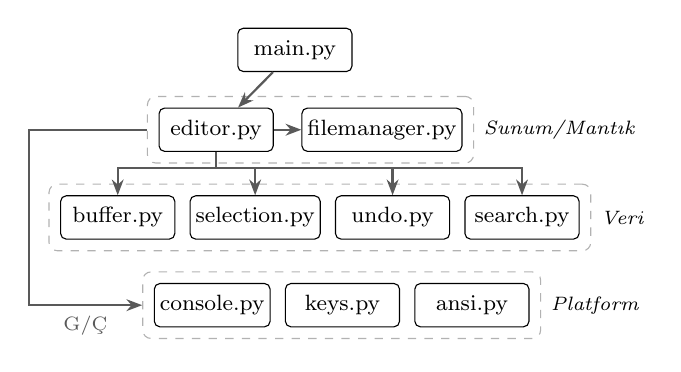
\begin{tikzpicture}[
  font=\footnotesize,
  mod/.style={draw, rounded corners=2pt, fill=white, minimum height=0.55cm, minimum width=1.45cm, inner sep=2pt},
  katman/.style={draw=gray!60, dashed, rounded corners=3pt, inner sep=4pt},
  ok/.style={-{Stealth[length=2mm]}, thick, gray!70!black}]
\node[mod] (main) {main.py};
\node[mod, below=0.45cm of main, xshift=-1.0cm] (ed) {editor.py};
\node[mod, right=0.35cm of ed] (fm) {filemanager.py};
\node[mod, below=0.55cm of ed, xshift=-1.25cm] (buf) {buffer.py};
\node[mod, right=0.18cm of buf] (sel) {selection.py};
\node[mod, right=0.18cm of sel] (und) {undo.py};
\node[mod, right=0.18cm of und] (sea) {search.py};
\node[mod, below=0.55cm of buf, xshift=1.2cm] (con) {console.py};
\node[mod, right=0.18cm of con] (key) {keys.py};
\node[mod, right=0.18cm of key] (ans) {ansi.py};
\node[katman, fit=(ed)(fm), label={[font=\scriptsize\itshape]right:Sunum/Mantık}] (k1) {};
\node[katman, fit=(buf)(sea), label={[font=\scriptsize\itshape]right:Veri}] (k2) {};
\node[katman, fit=(con)(ans), label={[font=\scriptsize\itshape]right:Platform}] (k3) {};
\draw[ok] (main) -- (ed);
\draw[ok] (ed) -- (fm);
\draw[ok] (ed.south) -- ++(0,-0.2) -| (buf.north);
\draw[ok] (ed.south) -- ++(0,-0.2) -| (sel.north);
\draw[ok] (ed.south) -- ++(0,-0.2) -| (und.north);
\draw[ok] (ed.south) -- ++(0,-0.2) -| (sea.north);
\draw[ok] (k1.west) -- (k1.west -| k2.west) -- ++(-0.25,0) |- node[pos=0.75, below, font=\scriptsize]{G/Ç} (k3.west);
\end{tikzpicture}
\caption{Uygulamanın katmanlı mimarisi ve modüller arası bağımlılıklar.}
\label{fig:mimari}
\end{figure}

\begin{table}[t]
\centering
\caption{Modüller ve Sorumlulukları}
\label{tab:moduller}
\begin{tabular}{@{}p{2.15cm}p{5.0cm}r@{}}
\toprule
\textbf{Modül} & \textbf{Sorumluluk} & \textbf{Satır} \\
\midrule
\kod{console.py} & Ham giriş, VT modu, tuş çözümleme, pano & 293 \\
\kod{keys.py} & Tuş olayı sınıfı (\kod{Key}) & 24 \\
\kod{ansi.py} & Renk kodları, konumlandırma, hizalama & 50 \\
\kod{buffer.py} & Metin veri yapısı (\kod{TextBuffer}) & 121 \\
\kod{selection.py} & Seçimin indekslerle takibi & 39 \\
\kod{undo.py} & \kod{Stack} ve \kod{Action} sınıfları & 59 \\
\kod{search.py} & KMP ve tüm eşleşmeleri bulma & 67 \\
\kod{filemanager.py} & Konsol içi dosya yöneticisi & 233 \\
\kod{editor.py} & Komutlar, tuş yönlendirme, çizim & 748 \\
\kod{main.py} & Giriş noktası, hata yakalama & 31 \\
\midrule
\multicolumn{2}{@{}l}{\textbf{Toplam}} & \textbf{1665} \\
\bottomrule
\end{tabular}
\end{table}

\subsection{Konsol Giriş/Çıkış Katmanı}

\textit{1) Ham giriş:} Python'un \kod{input()} fonksiyonu Enter beklediği ve değiştirici tuşları raporlamadığı için kullanılamaz. Bunun yerine konsol \kod{SetConsoleMode} \cite{msmode} ile satır tamponu (\kod{ENABLE\_LINE\_INPUT}), yankı (\kod{ENABLE\_ECHO\_INPUT}), \kod{Ctrl+C} sinyali (\kod{ENABLE\_PROCESSED\_INPUT}), fare girişi ve fare ile hızlı düzenleme (\kod{QUICK\_EDIT}) kapatılarak ham moda alınmıştır. Fare girişinin kapatılması projenin ``fare kullanılmayacaktır'' şartını işletim sistemi seviyesinde garanti eder. Ardından her tuş olayı \kod{ReadConsoleInputW} \cite{msinput} ile bir \kod{INPUT\_RECORD} yapısı olarak okunur. Bu yapı, sanal tuş kodu (VK), donanım tarama kodu, Unicode karakter ve Ctrl/Alt/Shift durum bayraklarını içerir. Yapıların Python tarafındaki karşılıkları \kod{ctypes.Structure} ile tanımlanmış; \kod{KEY\_EVENT\_RECORD} için 16, \kod{INPUT\_RECORD} için 20 baytlık Windows bellek düzeninin birebir sağlandığı doğrulanmıştır.

\textit{2) Tuş çözümleme:} Ham olaylar Tablo~\ref{tab:tus} üzerindeki kurallarla platformdan bağımsız \kod{Key} nesnelerine dönüştürülür. Burada iki özel durum önemlidir. Birincisi, Türkçe Q klavyede \kod{@ \# \{ \} [ ] \textbackslash\ |} karakterleri AltGr tuşuyla yazılır ve Windows AltGr'yi ``Ctrl+Alt'' olarak bildirir. Ctrl'ye basılı her olay kısayol sayılsaydı bu karakterler yazılamazdı; bu nedenle Ctrl ile birlikte Alt da basılıysa olay normal karakter olarak yorumlanır. İkincisi, ASCII tablosunda \kod{Ctrl+H} ile Backspace aynı koda (8) karşılık gelir ve bazı terminal öykünücüleri \kod{Ctrl+H}'yi Backspace olarak iletir. Bu durum, H tuşunun tarama kodu (0x23) ve klasik konsolda gerçek \kod{Ctrl+Backspace}'in \kod{0x7F} karakteri üretmesi kullanılarak ayırt edilmiştir.

\begin{table}[t]
\centering
\caption{Tuş Olaylarının Çözümlenme Kuralları (Öncelik Sırasıyla)}
\label{tab:tus}
\begin{tabular}{@{}cp{3.6cm}p{2.9cm}@{}}
\toprule
\textbf{\#} & \textbf{Koşul} & \textbf{Sonuç} \\
\midrule
1 & VK=Backspace ve (tarama=0x23 veya Ctrl+\kod{\textbackslash x08}) & \kod{Ctrl+H} \\
2 & VK özel tuş tablosunda & Yön, Enter, ESC, \ldots \\
3 & Yazılabilir karakter ve (Ctrl yok veya Alt var) & \kod{CHAR} (AltGr dahil) \\
4 & Ctrl basılı ve VK $\in$ [A--Z] & \kod{Ctrl+harf} \\
5 & VK=0 ve karakter \kod{\textbackslash r} / \kod{\textbackslash t} & Enter / Tab (yapıştırma) \\
6 & Diğer (yalnız Shift, Ctrl, \ldots) & Yok sayılır \\
\bottomrule
\end{tabular}
\end{table}

\textit{3) Çıkış ve VT dizileri:} Renkler ve imleç kontrolü için çıkış tamponunda \kod{ENABLE\_VIRTUAL\_TERMINAL\_PROCESSING} bayrağı açılarak ECMA-48 standardındaki ANSI kaçış dizileri kullanılmıştır \cite{ecma48,msvt}. Kullanılan diziler Tablo~\ref{tab:vt} üzerinde verilmiştir. İmlecin proje tanımında istenen ``yanıp sönen dikey çizgi'' biçimi DECSCUSR dizisi (\kod{ESC[5~q}) ile, beyaz rengi ise OSC~12 dizisi ile ayarlanır. Uygulama alternatif ekran tamponunda çalıştığından, çıkışta kullanıcının konsoldaki önceki içeriği bozulmadan geri gelir. Metin \kod{WriteConsoleW} ile UTF-16 olarak yazıldığı ve kod sayfası 65001'e (UTF-8) ayarlandığı için Türkçe karakterler doğru görüntülenir.

\begin{table}[t]
\centering
\caption{Kullanılan ANSI/VT Kaçış Dizileri}
\label{tab:vt}
\begin{tabular}{@{}ll@{}}
\toprule
\textbf{Dizi} & \textbf{Görevi} \\
\midrule
\kod{ESC[?1049h / l} & Alternatif ekran tamponuna geç / dön \\
\kod{ESC[?7l} & Satır sonunda otomatik kaydırmayı kapat \\
\kod{ESC[5~q} & İmleç: yanıp sönen dikey çizgi \\
\kod{ESC]12;\#ffffff BEL} & İmleç rengi: beyaz \\
\kod{ESC[?25l / h} & Çizim sırasında imleci gizle / göster \\
\kod{ESC[\textit{s};\textit{k}H} & İmleci $s$. satır, $k$. sütuna taşı \\
\kod{ESC[K} & Satırın kalanını temizle \\
\kod{ESC[30;103m} & Seçim: sarı arka plan \\
\kod{ESC[97;44m} & Arama eşleşmesi: mavi arka plan \\
\bottomrule
\end{tabular}
\end{table}

\subsection{Metin Veri Yapısı}

Proje tanımı, metindeki her karakterin seçilen bir veri yapısında tutulmasını ve dosya içeriğinin dinamik olarak yönetilmesini istemektedir. Bu amaçla iki seviyeli bir yapı seçilmiştir: $n$ satırlık bir metin $L = [\ell_0, \ell_1, \ldots, \ell_{n-1}]$ dinamik listesiyle, her satır da $\ell_i = [c_0, c_1, \ldots, c_{m_i-1}]$ karakter listesiyle temsil edilir. Satır sonu karakterleri saklanmaz; satırlar arası sınır liste yapısının kendisiyle ifade edilir. Böylece bir satırın numarası her zaman o satırın liste indeksinin bir fazlasıdır ve satır eklendiğinde ya da silindiğinde numaralar ek bir işlem gerekmeden kendiliğinden güncellenir.

Tüm düzenleme işlemleri yalnızca iki temel fonksiyondan geçer: \kod{insert\_text(r, c, metin)} ve \kod{delete\_range(başlangıç, bitiş)}. Çok satırlı ekleme sırasında imlecin sağında kalan kuyruk kesilir, metnin ilk parçası satıra eklenir, kalan parçalar yeni satırlar olarak araya yerleştirilir ve kuyruk son satırın sonuna eklenir. Silme işlemi ise ilk satırın başı ile son satırın kuyruğunu birleştirip aradaki satırları kaldırır. Silinen metin geri alma işlemi için çağırana döndürülür.

\begin{table}[t]
\centering
\caption{Metin Veri Yapılarının Asimptotik Karşılaştırması}
\label{tab:veriyapisi}
\setlength{\tabcolsep}{4pt}
\begin{tabular}{@{}lccc@{}}
\toprule
\textbf{Yapı} & \textbf{Erişim} & \textbf{Düzenleme} & \textbf{Zorluk} \\
\midrule
Tek parça dizi & $O(N)$ & $O(N)$ & Düşük \\
Karakter bağlı listesi & $O(N)$ & $O(1)$\textsuperscript{\dag} & Orta \\
Gap buffer \cite{finseth} & $O(N)$ & $O(1)$\textsuperscript{\ddag} & Orta \\
Piece table \cite{crowley} & $O(p)$ & $O(p)$ & Yüksek \\
\textbf{Satır listesi (seçilen)} & $\mathbf{O(1)}$ & $\mathbf{O(m)}$ & \textbf{Düşük} \\
\bottomrule
\multicolumn{4}{@{}p{8.2cm}@{}}{\footnotesize Erişim: $(r,c)$ konumuna ulaşma. $N$: toplam karakter, $m$: satır uzunluğu, $p$: parça sayısı. \textsuperscript{\dag}Konum bilindiğinde. \textsuperscript{\ddag}Amortize, boşluk imleçteyken.}
\end{tabular}
\end{table}

Tablo~\ref{tab:veriyapisi}, seçilen yapıyı yaygın alternatiflerle karşılaştırmaktadır. Tek parça bir dizide dosyanın ortasına yapılan her ekleme, ekleme noktasından sonraki tüm karakterlerin kaydırılmasını gerektirir. Karakterlerin bağlı listede tutulması eklemeyi sabit zamana indirse de, $(r,c)$ konumuna ulaşmak için listenin baştan dolaşılması gerekir; ekran çizimi ve imleç hareketi gibi en sık yapılan işlemler bu nedenle yavaşlar. Gap buffer ve piece table ise yüksek başarımlı editörlerde kullanılan ancak gerçeklemesi daha karmaşık yapılardır. Bir metin editöründe düzenlemeler neredeyse her zaman tek bir satırda yoğunlaştığı ve satırlar genellikle kısa olduğu için ($m \ll N$), satır listesi yapısı hem $O(1)$ erişim hem de $O(m)$ düzenleme maliyetiyle bu proje için en dengeli seçenektir. Bu öngörü Bölüm~\ref{sec:deney}'te deneysel olarak doğrulanmıştır.

\subsection{Seçim ve İndeks Dönüşümü}

Proje tanımı gereği seçili metin, başlangıç ve bitiş indeksleriyle takip edilir. \kod{Selection} sınıfında \kod{start} seçimin başladığı sabit indeksi, \kod{end} ise imlecin hareketli indeksini tutar. Kullanıcı sola doğru seçim yaptığında $\mathit{end} < \mathit{start}$ olabileceğinden, kullanım anında $[\min, \max)$ aralığı hesaplanır. Doğrusal indeks ile $(r,c)$ konumu arasındaki dönüşüm, her satır sonundaki ayırıcı da bir karakter sayılarak (\ref{eq:indeks}) ile yapılır:
\begin{equation}
\mathrm{idx}(r,c) = \sum_{k=0}^{r-1}\left(|\ell_k| + 1\right) + c
\label{eq:indeks}
\end{equation}
Ters dönüşüm, indeksten satır uzunluklarını sırayla çıkararak yapılır. \kod{Ctrl+Yön} karakter karakter, \kod{Ctrl+Shift+Yön} ise kelime kelime seçim yapar. Kelime sınırları karakterler üç sınıfa ayrılarak belirlenir: kelime karakteri (harf, rakam, alt çizgi; Türkçe harfler \kod{isalnum()} ile doğru tanınır), boşluk ve noktalama. Sağa kelime hareketi önce aynı sınıftaki ardışık karakterleri, sonra boşlukları atlar; sola hareket bunun tersini uygular. Satır başında ya da sonunda hareket bir önceki ya da sonraki satıra geçer. Seçim aktifken yazılan bir karakter, Backspace ya da yapıştırma işlemi önce seçili metni siler.

\subsection{Geri Alma (Undo) Mekanizması}

Geri alma için en basit yöntem her düzenlemeden önce metnin tam bir kopyasını (anlık görüntü) saklamaktır; ancak bu yöntemin bellek maliyeti $O(N \cdot k)$'dir ($k$: düzenleme sayısı). Bu projede bunun yerine Komut (Command) tasarım deseninden \cite{gof} esinlenen işlem tabanlı bir yaklaşım kullanılmıştır. Yığına yalnızca yapılan işlem kaydedilir ve geri alma işlemi bu kaydın tersini uygular:

\begin{itemize}
\item \kod{INSERT}$(p, t)$: $p$ konumuna $t$ eklendi. Tersi: $p$ ile $\mathrm{son}(p,t)$ arası silinir.
\item \kod{DELETE}$(p, t)$: $p$ konumundan $t$ silindi. Tersi: $t$, $p$ konumuna eklenir.
\item \kod{BATCH}$(a_1, \ldots, a_k)$: Toplu işlem. Tersi: alt işlemler $a_k, \ldots, a_1$ sırasıyla geri alınır.
\end{itemize}

Yığın, Python listesi üzerinde \kod{push}, \kod{pop}, \kod{peek}, \kod{is\_empty} ve \kod{size} işlemlerine sahip özgün bir \kod{Stack} sınıfı olarak tasarlanmıştır; tüm işlemler $O(1)$'dir. Yığın 1000 kayıtla sınırlandırılmış, sınır aşıldığında en eski kayıt atılmaktadır. Her karakter için ayrı bir kayıt tutulması kullanıcının bir kelimeyi silmek için defalarca \kod{Ctrl+Z}'ye basmasına yol açacağından, ardışık ve bitişik karakter eklemeleri tek bir \kod{INSERT} kaydında birleştirilir. Boşluk karakteri, imleç hareketi, silme ya da kaydetme işlemi birleştirmeyi sonlandırır; böylece geri alma kelime kelime çalışır.

Dosyanın kaydedilip kaydedilmediği de geri alma yığını üzerinden belirlenir. Her \kod{Action} nesnesine benzersiz bir numara verilir; kaydetme anında yığının tepesindeki kaydın numarası saklanır. Dosya, ancak yığının o anki tepe numarası bu değerden farklıysa ``değiştirilmiş'' sayılır. Bu yöntem sayesinde kullanıcı kayıttan sonra bir değişiklik yapıp geri aldığında, çıkışta gereksiz yere ``Kaydetmek istiyor musunuz?'' sorusu sorulmaz. Geri alma algoritması Algoritma~\ref{alg:undo} üzerinde verilmiştir.

\begin{algorithm}[t]
\caption{Geri Alma}
\label{alg:undo}
\begin{algorithmic}[1]
\Procedure{GeriAl}{}
  \State $a \gets$ \Call{Yığın.Pop}{}
  \If{$a = \textsc{Boş}$} \State \Return ``Geri alınacak işlem yok''
  \EndIf
  \State \Call{TersUygula}{$a$}
  \State İmleci $a.\mathit{imleç\_önce}$ konumuna taşı; seçimi temizle
\EndProcedure
\Procedure{TersUygula}{$a$}
  \If{$a.\mathit{tür} = \textsc{Insert}$}
    \State \Call{Sil}{$a.p,\ \textsc{Son}(a.p, a.t)$}
  \ElsIf{$a.\mathit{tür} = \textsc{Delete}$}
    \State \Call{Ekle}{$a.p,\ a.t$}
  \Else \Comment{\textsc{Batch}}
    \For{$i \gets k$ \textbf{down to} $1$}
      \State \Call{TersUygula}{$a.\mathit{alt}_i$}
    \EndFor
  \EndIf
\EndProcedure
\end{algorithmic}
\end{algorithm}

\subsection{Arama: Knuth-Morris-Pratt Algoritması}

Proje tanımı, arama işlemlerinin bir string eşleşme algoritmasıyla yapılmasını istemektedir. Naif arama, bir uyuşmazlıkta metinde geri dönerek bir sonraki konumdan yeniden başladığı için en kötü durumda $O(n \cdot m)$ zaman alır ($n$: metin, $m$: aranan kelime uzunluğu). KMP algoritması \cite{kmp,clrs} ise aranan kelimenin kendi içindeki tekrarları önceden LPS (\textit{Longest Proper Prefix which is also Suffix}) tablosunda hesaplar. $\mathrm{lps}[i]$, kelimenin ilk $i+1$ karakterinde hem önek hem sonek olan en uzun özel parçanın uzunluğudur. Bir uyuşmazlık olduğunda metindeki konum hiç geri alınmaz; yalnızca kelimedeki konum $\mathrm{lps}$ değerine çekilir. Böylece toplam süre $O(n + m)$ olur. Örneğin ``ABABCABAB'' kelimesi için LPS tablosu $[0,0,1,2,0,1,2,3,4]$ şeklindedir. Algoritma~\ref{alg:kmp}, gerçeklenen arama yordamını göstermektedir.

\begin{algorithm}[t]
\caption{KMP ile Tüm Eşleşmeleri Bulma}
\label{alg:kmp}
\begin{algorithmic}[1]
\Require Metin $T[0..n-1]$, kelime $P[0..m-1]$
\Ensure Eşleşmelerin başlangıç indeksleri
\State $\mathrm{lps} \gets$ \Call{LPSOluştur}{$P$}; \ $S \gets \emptyset$
\State $i \gets 0$; \ $j \gets 0$
\While{$i < n$}
  \If{$T[i] = P[j]$}
    \State $i \gets i+1$; \ $j \gets j+1$
    \If{$j = m$}
      \State $S \gets S \cup \{i - j\}$; \ $j \gets \mathrm{lps}[j-1]$
    \EndIf
  \ElsIf{$j > 0$}
    \State $j \gets \mathrm{lps}[j-1]$ \Comment{$i$ geri gitmez}
  \Else
    \State $i \gets i+1$
  \EndIf
\EndWhile
\State \Return $S$
\end{algorithmic}
\end{algorithm}

KMP doğası gereği çakışan eşleşmeleri de bulur (``aaaa'' içinde ``aa'' için 0, 1 ve 2). Değiştirme işleminin tutarlı olması için \kod{find\_all} fonksiyonu her satırda eşleşmeleri soldan sağa tarar ve bir önceki eşleşmenin bitişinden önce başlayanları eler. Aranan kelimeler satır sınırını aşamayacağından arama her satıra ayrı ayrı uygulanır; sonuç, $(r,c)$ sırasına göre sıralı bir liste olarak döner.

Arama ile ilgili üç kısayol bulunmaktadır. \kod{Ctrl+F}'de kullanıcı yazdıkça arama yeniden yapılır ve tüm eşleşmeler anlık olarak mavi arka planla gösterilir; Enter ile onaylandığında imleç imlece en yakın sonraki eşleşmeye taşınır. \kod{Ctrl+G}'de tüm eşleşmeler bulunduktan sonra kullanıcı sağ/aşağı yön tuşlarıyla sonraki, sol/yukarı tuşlarıyla önceki eşleşmeye geçer. Geçiş $i \gets (i \pm 1) \bmod k$ ile yapıldığından sondan sonra başa dönülür; o an üzerinde durulan eşleşme açık mavi ile ayrıca vurgulanır. \kod{Ctrl+H} ise bir sonraki alt bölümde açıklanmıştır.

\subsection{Toplu Değiştirme}

\kod{Ctrl+H} ile önce değiştirilecek kelime, ardından yeni kelime girilir; her iki aşamada da ESC işlemi iptal eder. Değiştirme sırasında yapılan bir silme işlemi, aynı satırdaki sonraki eşleşmelerin sütun numaralarını kaydırır. Bu sorunu ek hesaplama yapmadan çözmek için eşleşmeler sondan başa doğru işlenir: sondaki bir eşleşmenin değiştirilmesi, kendisinden önceki eşleşmelerin konumunu etkilemez (Algoritma~\ref{alg:replace}). Tüm alt işlemler tek bir \kod{BATCH} kaydında toplandığından, yüzlerce değişiklik tek bir \kod{Ctrl+Z} ile geri alınabilir.

\begin{algorithm}[t]
\caption{Tümünü Değiştir}
\label{alg:replace}
\begin{algorithmic}[1]
\Require Eski kelime $e$, yeni kelime $y$
\State $M \gets$ \Call{TümEşleşmeler}{$e$} \Comment{$(r,c)$'ye göre sıralı}
\State \Call{TopluİşlemBaşlat}{}
\For{$(r,c) \in M$ \textbf{sondan başa}}
  \State \Call{Sil}{$(r,c),\ (r, c+|e|)$}
  \If{$y \neq \varepsilon$} \State \Call{Ekle}{$(r,c),\ y$}
  \EndIf
\EndFor
\State \Call{TopluİşlemBitir}{} \Comment{tek \textsc{Batch} kaydı}
\State \Return $|M|$
\end{algorithmic}
\end{algorithm}

\subsection{Dosya İşlemleri ve Dosya Yöneticisi}

Dosya Aç (\kod{Ctrl+O}), Dosya Kaydet (\kod{Ctrl+S}) ve Dosya Farklı Kaydet (\kod{Ctrl+Shift+S}) komutları konsol içinde çalışan bir dosya yöneticisi açar. Yönetici, mevcut dosya varsa onun bulunduğu dizinden, yoksa programın çalıştırıldığı dizinden başlar. Listenin başında üst dizini temsil eden ``..'' öğesi yer alır; ardından klasörler ve dosyalar büyük/küçük harf duyarsız alfabetik sırayla listelenir. Yukarı/aşağı tuşları öğeler arasında gezinmeyi, sağ ok (\textit{ileri}) seçili klasörün içine girmeyi, sol ok (\textit{geri}) ise üst dizine çıkmayı sağlar. Üst dizine çıkıldığında imleç az önce çıkılan klasörün üzerine konumlandırılır. Kullanıcı dosya adını yazar ve Enter ile işlemi tamamlar; ESC işlemi iptal eder. Açma modunda listede bir dosyanın üzerine gelindiğinde adı otomatik olarak giriş alanına yazılır. Kaydetme modunda var olan bir dosyanın adı girilirse üzerine yazma için onay istenir. Erişim izni olmayan klasörler hata mesajıyla bildirilir ve uygulama çökmez.

Proje tanımı gereği \kod{Ctrl+S}, dosya daha önce kaydedilmişse dosya yöneticisini açmadan doğrudan aynı yola kaydeder. Dosyalar UTF-8 olarak kaydedilir. Açarken önce UTF-8 (BOM dahil) denenir; başarısız olursa Türkçe Windows kod sayfası olan CP-1254 kullanılır. Böylece eski Windows uygulamalarıyla oluşturulmuş Türkçe dosyalar da bozulmadan açılır.

\kod{ESC} tuşu ile çıkılmak istendiğinde dosya kaydedilmemişse ``Kaydetmek istiyor musunuz? (y/n)'' sorusu sorulur. \kod{y} yanıtında dosya kaydedilir ve çıkılır; dosyanın daha önce bir yolu yoksa dosya yöneticisi açılır, kullanıcı burada iptal ederse çıkış da iptal edilir. \kod{n} yanıtında değişiklikler kaydedilmeden çıkılır. Arama vurgusu açıkken basılan ilk ESC yalnızca vurguyu kaldırır; bu sayede kullanıcı aramayı kapatmak isterken yanlışlıkla çıkış yapmaz. Benzer şekilde, değişiklik yapılmış bir dosya açıkken yeni bir dosya açılmak istenirse önce kaydetme sorusu sorulur.

\subsection{Ekran Çizimi}

Ekran yukarıdan aşağıya şu bölgelerden oluşur: toolbox şeridi, ayırıcı çizgi, satır numaralı metin alanı, durum çubuğu ve mesaj/giriş satırı. Her tuş işlendikten sonra tüm ekran tek bir karakter dizisi olarak oluşturulup tek bir \kod{WriteConsoleW} çağrısıyla yazılır. Çizim süresince imlecin gizlenmesi ve her satırın kendi konumuna doğrudan yazılması titremeyi önler.

\textit{1) Toolbox şeridi:} Her komut ``Ad (Kısayol)'' biçiminde bir parçaya dönüştürülür. Parçalar açgözlü (greedy) satır kırma yöntemiyle yan yana dizilir: bir sonraki parça mevcut satıra sığmıyorsa yeni bir satıra geçilir. Böylece proje tanımında istendiği gibi seçenekler aynı satırda yan yana dizilir ve sığmadığında ikinci satırdan devam eder. Pencere boyutu değiştiğinde şerit yeniden hesaplanır.

\textit{2) Görünüm penceresi:} İmleç her zaman görünür olacak şekilde dikey (\kod{top}) ve yatay (\kod{left}) kaydırma değerleri güncellenir. Satır numarası sütununun genişliği satır sayısının basamak sayısına göre dinamik olarak hesaplanır.

\textit{3) Renklendirme:} Görünen her satır için karakter başına bir stil dizisi oluşturulur. Önce arama eşleşmeleri mavi, ardından seçim sarı olarak işaretlenir; seçim aramanın üzerine yazar. Ardışık aynı stildeki karakterler tek bir kaçış dizisiyle gruplanır. Seçim bir satırın sonunu kapsıyorsa, satır sonu karakterinin de seçildiğini göstermek için satırın sonuna sarı bir boşluk çizilir.

\textit{4) Ertelenmiş çizim:} Ana döngü, çizimden önce \kod{PeekConsoleInputW} ile kuyrukta işlenecek başka bir tuş olup olmadığını kontrol eder. Kuyrukta tuş varsa çizim atlanır. Bu sayede panodan büyük bir metin yapıştırıldığında ya da bir tuş basılı tutulduğunda yüzlerce ara kare yerine yalnızca son durum çizilir. Uygulamanın ana döngüsü Şekil~\ref{fig:akis} üzerinde gösterilmiştir.

\begin{figure}[t]
\centering
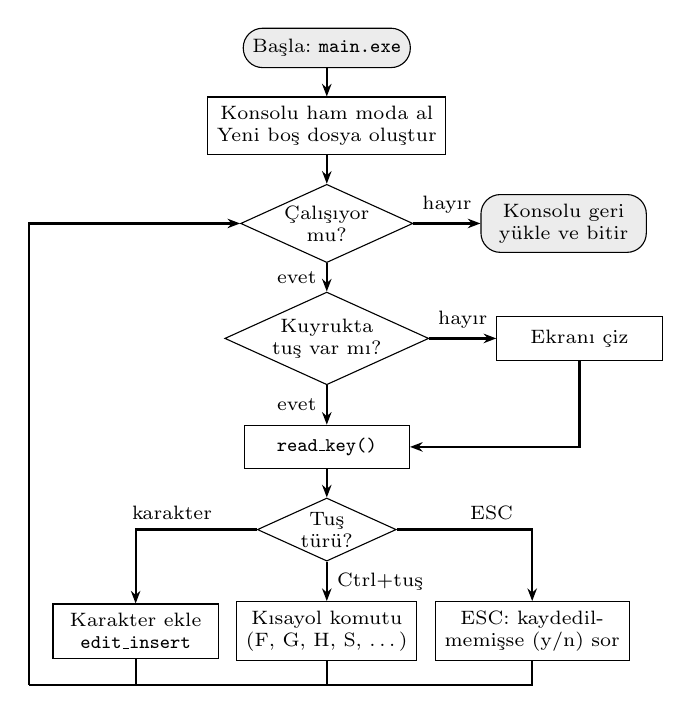
\begin{tikzpicture}[
  font=\scriptsize, node distance=0.36cm,
  basla/.style={draw, rounded corners=7pt, fill=gray!15, minimum width=2.1cm, minimum height=0.5cm, align=center},
  islem/.style={draw, fill=white, minimum width=2.1cm, minimum height=0.55cm, align=center},
  karar/.style={draw, diamond, aspect=2.2, fill=white, inner sep=0.5pt, align=center},
  ok/.style={-{Stealth[length=1.6mm]}, thick}]
\node[basla] (bas) {Başla: \kod{main.exe}};
\node[islem, below=of bas] (init) {Konsolu ham moda al\\Yeni boş dosya oluştur};
\node[karar, below=of init] (calis) {Çalışıyor\\mu?};
\node[basla, right=0.85cm of calis] (son) {Konsolu geri\\yükle ve bitir};
\node[karar, below=of calis] (bek) {Kuyrukta\\tuş var mı?};
\node[islem, right=0.85cm of bek] (ciz) {Ekranı çiz};
\node[islem, below=0.5cm of bek] (oku) {\kod{read\_key()}};
\node[karar, below=of oku] (tur) {Tuş\\türü?};
\node[islem, below=0.5cm of tur] (kis) {Kısayol komutu\\(F, G, H, S, \ldots)};
\node[islem, left=0.22cm of kis] (yaz) {Karakter ekle\\\kod{edit\_insert}};
\node[islem, right=0.22cm of kis] (esc) {ESC: kaydedil-\\memişse (y/n) sor};
\draw[ok] (bas) -- (init);
\draw[ok] (init) -- (calis);
\draw[ok] (calis) -- node[above]{hayır} (son);
\draw[ok] (calis) -- node[left]{evet} (bek);
\draw[ok] (bek) -- node[above]{hayır} (ciz);
\draw[ok] (ciz) |- (oku);
\draw[ok] (bek) -- node[left]{evet} (oku);
\draw[ok] (oku) -- (tur);
\draw[ok] (tur.west) -| node[above, pos=0.35]{karakter} (yaz.north);
\draw[ok] (tur) -- node[right]{Ctrl+tuş} (kis);
\draw[ok] (tur.east) -| node[above, pos=0.35]{ESC} (esc.north);
\coordinate (alt) at ($(kis.south)+(0,-0.3)$);
\coordinate (L) at ($(yaz.west)+(-0.3,0)$);
\draw[thick] (yaz.south) -- (yaz.south |- alt);
\draw[thick] (kis.south) -- (alt);
\draw[thick] (esc.south) -- (esc.south |- alt) -- (L |- alt);
\draw[ok] (L |- alt) -- (L |- calis) -- (calis.west);
\end{tikzpicture}
\caption{Uygulamanın ana döngüsüne ait akış diyagramı.}
\label{fig:akis}
\end{figure}

% ================================================================ DENEYSEL SONUÇLAR
\section{Deneysel Sonuçlar}\label{sec:deney}

\subsection{Test Yöntemi}

Mimarideki bağımlılık enjeksiyonu sayesinde editör, gerçek Windows konsolu yerine önceden belirlenmiş bir tuş dizisini sırayla döndüren ve çizilen son ekran karesini kaydeden sahte bir konsol nesnesiyle çalıştırılabilmektedir. Bu yöntemle uygulama, uçtan uca kullanım senaryoları üzerinden otomatik olarak test edilmiştir. Her senaryo bir tuş dizisi ile başlar (örneğin ``metin yaz, \kod{Ctrl+H}'ye bas, eski kelimeyi yaz, Enter, yeni kelimeyi yaz, Enter, \kod{Ctrl+Z}'ye bas'') ve sonunda metin içeriği, imleç konumu, pano içeriği, diske yazılan dosyanın içeriği ya da ekran karesindeki renk kodları beklenen değerlerle karşılaştırılır. Platform katmanı ise Windows 11 klasik konsolunda (conhost) elle test edilmiştir. Başarım ölçümleri Python 3.12 ile x86-64 bir test ortamında, her ölçüm en az üç kez tekrarlanıp en iyi süre alınarak yapılmıştır; ölçüm betiği (\kod{bench.py}) proje dosyalarıyla birlikte verilmiştir.

\subsection{Fonksiyonel Testler}

Toplam 36 otomatik test senaryosunun tamamı başarıyla geçmiştir. Senaryoların kategorilere göre dağılımı Tablo~\ref{tab:testler} üzerinde, proje tanımındaki gereksinimlerin karşılanma durumu ise Tablo~\ref{tab:gereksinim} üzerinde verilmiştir.

\begin{table}[t]
\centering
\caption{Otomatik Test Senaryoları}
\label{tab:testler}
\begin{tabular}{@{}p{2.6cm}p{4.2cm}c@{}}
\toprule
\textbf{Kategori} & \textbf{Doğrulanan davranışlar} & \textbf{Sonuç} \\
\midrule
Algoritma & LPS tablosu, KMP (çakışan eşleşmeler dahil) & 2/2 \\
Yazma ve silme & Türkçe karakter, Backspace, Ctrl+Backspace, satır birleştirme & 3/3 \\
Seçim ve pano & Karakter/kelime seçimi (iki yön), kopyala, kes, yapıştır, seçimin üzerine yazma, çok satırlı seçim & 5/5 \\
Geri alma & Kelime bazlı geri alma, tümünü geri alma, silme geri alma & 3/3 \\
Arama ve değiştirme & Ctrl+F vurgusu, ESC davranışı, Ctrl+G ileri/geri ve başa dönme, Ctrl+H, iki aşamada ESC ile iptal, tek adımda geri alma & 8/8 \\
Ekran & Satır numarası artışı/azalışı, toolbox, sarı seçim, dikey kaydırma & 5/5 \\
Dosya işlemleri & Yeni kaydetme, tekrar kaydetme, alt klasöre kaydetme, geri gitme, üzerine yazma onayı, açma & 6/6 \\
Çıkış & Temiz çıkış, (y/n) sorusu, \kod{n}, \kod{y} ile kaydedip çıkma & 4/4 \\
\midrule
\textbf{Toplam} & & \textbf{36/36} \\
\bottomrule
\end{tabular}
\end{table}

\begin{table}[t]
\centering
\caption{Proje Gereksinimlerinin Karşılanma Durumu}
\label{tab:gereksinim}
\begin{tabular}{@{}p{4.9cm}p{2.6cm}@{}}
\toprule
\textbf{Gereksinim} & \textbf{Gerçekleme} \\
\midrule
\kod{main.exe} ile yeni boş dosya açılması & PyInstaller, \kod{main.py} \\
Toolbox, kısayollar parantez içinde, taşma & Açgözlü satır kırma \\
Fare kullanılmaması & Fare girişi kapalı \\
Yanıp sönen beyaz dikey imleç & DECSCUSR + OSC 12 \\
Türkçe karakter desteği & UTF-16 G/Ç, CP-1254 \\
Dosya yöneticisi, ileri/geri, Enter & \kod{filemanager.py} \\
Kayıtlı dosyada Ctrl+S'nin yönetici açmaması & \kod{cmd\_save} \\
Ctrl+F mavi vurgu & KMP + ANSI 44 \\
Ctrl+G eşleşmeler arası gezinme & Modüler indeks \\
Ctrl+H tümünü değiştir, ESC iptal & Sondan başa, \textsc{Batch} \\
Ctrl+Yön / Ctrl+Shift+Yön seçimi, sarı & \kod{Selection}, ANSI 103 \\
Ctrl+C / X / V / Z & Pano + \kod{Stack} \\
Backspace / Ctrl+Backspace & Karakter / kelime silme \\
Dinamik satır numaraları & Liste indeksi + 1 \\
ESC ile çıkış, (y/n) sorusu & \kod{cmd\_exit} \\
Karakterlerin veri yapısında tutulması & Satır listesi \\
Undo için stack yapısı & Özgün \kod{Stack} sınıfı \\
Seçimin indekslerle takibi & \kod{start}/\kod{end} \\
String eşleşme algoritması & KMP \\
Harici GUI kütüphanesi kullanılmaması & Yalnız standart kütüphane \\
\bottomrule
\end{tabular}
\end{table}

\subsection{Ekran Görüntüleri}

Şekil~\ref{fig:ekran-editor}, \ref{fig:ekran-replace} ve \ref{fig:ekran-fm}'de uygulamanın farklı durumlardaki ekranları verilmiştir. Bu görüntüler, editörün konsola gönderdiği karakter ve renk kodlarından birebir üretilmiştir. Şekil~\ref{fig:ekran-editor}'de ``editör'' kelimesine ait arama eşleşmeleri mavi, \kod{Ctrl+Shift+Sağ} ile seçilen iki kelime sarı arka planla görülmekte; durum çubuğu seçimin 13 karakter olduğunu göstermektedir.

\begin{figure*}[t]
\centering
\ekran{shot_editor.tex}{7.2pt}
\caption{Editörün ana ekranı: toolbox şeridi, satır numaraları, mavi arama eşleşmeleri, sarı seçim ve durum çubuğu.}
\label{fig:ekran-editor}
\end{figure*}

\begin{figure*}[t]
\centering
\ekran{shot_replace.tex}{7.2pt}
\caption{Ctrl+H ile değiştirme: aranan kelimenin eşleşmeleri vurgulanırken alt satırda yeni kelime isteniyor.}
\label{fig:ekran-replace}
\end{figure*}

\begin{figure*}[t]
\centering
\ekran{shot_fm.tex}{7.2pt}
\caption{Dosya Kaydet sırasında açılan konsol içi dosya yöneticisi: klasörler, dosya boyutları, kısayol yardımı ve dosya adı giriş alanı.}
\label{fig:ekran-fm}
\end{figure*}

\subsection{Başarım Ölçümleri}

\textit{1) Ekleme maliyeti:} Bölüm~\ref{sec:yontem}'deki veri yapısı tercihini sınamak için dosyanın ortasına 1000 karakter eklenmiş ve işlem başına süre ölçülmüştür. Karşılaştırma için metnin tek parça bir string olarak tutulduğu yapı kullanılmıştır. Şekil~\ref{fig:ekleme}'de görüldüğü gibi tek parça yapıda maliyet dosya boyutuyla doğrusal arttığı hâlde, satır listesi yapısında dosya boyutundan bağımsız olarak yaklaşık 3~$\mu$s'de sabit kalmaktadır. 50.000 satırlık (yaklaşık 4 MB) bir dosyada satır listesi yapısı yaklaşık 2400 kat daha hızlıdır.

\begin{figure}[t]
\centering
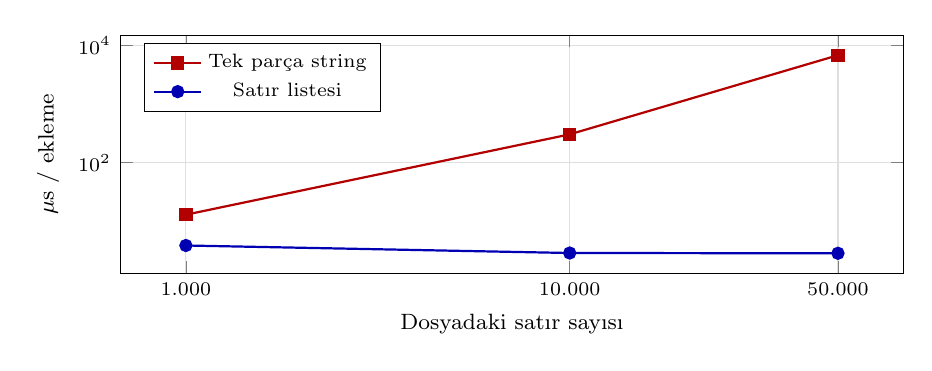
\begin{tikzpicture}
\begin{axis}[
  width=0.95\columnwidth, height=4.6cm,
  xmode=log, ymode=log,
  xlabel={Dosyadaki satır sayısı}, ylabel={$\mu$s / ekleme},
  xtick={1000,10000,50000}, xticklabels={1.000,10.000,50.000},
  legend style={font=\scriptsize, at={(0.03,0.97)}, anchor=north west},
  tick label style={font=\scriptsize}, label style={font=\footnotesize},
  grid=major, grid style={gray!25}]
\addplot[mark=square*, thick, red!70!black] coordinates {(1000,12.98) (10000,304.88) (50000,6833.25)};
\addplot[mark=*, thick, blue!70!black] coordinates {(1000,3.87) (10000,2.88) (50000,2.85)};
\legend{Tek parça string, Satır listesi}
\end{axis}
\end{tikzpicture}
\caption{Dosyanın ortasına karakter eklemenin işlem başına maliyeti (log--log ölçek).}
\label{fig:ekleme}
\end{figure}

\textit{2) Arama:} KMP ile naif arama, naif algoritmanın en kötü durumunu oluşturan bir girdi üzerinde karşılaştırılmıştır: yalnızca ``a'' karakterlerinden oluşan bir metinde, 49 adet ``a'' ve bir ``b''den oluşan ($m=50$) kelime aranmıştır. Bu girdide naif algoritma her konumda 50 karakter karşılaştırıp başarısız olurken KMP metinde hiç geri dönmez. Sonuçlar Şekil~\ref{fig:kmp}'de verilmiştir: KMP her boyutta yaklaşık 18 kat daha hızlıdır ve her iki algoritmanın süresi de beklendiği gibi $n$ ile doğrusal artmaktadır (naif algoritmanın çarpanı $m$'dir). Gerçekçi bir metinde (satır başına 10 kelime) \kod{find\_all} fonksiyonu 1.000 satırı 10,5~ms'de, 10.000 satırı (0,81 milyon karakter) 99~ms'de, 50.000 satırı (4,04 milyon karakter) ise 502~ms'de taramıştır.

\begin{figure}[t]
\centering
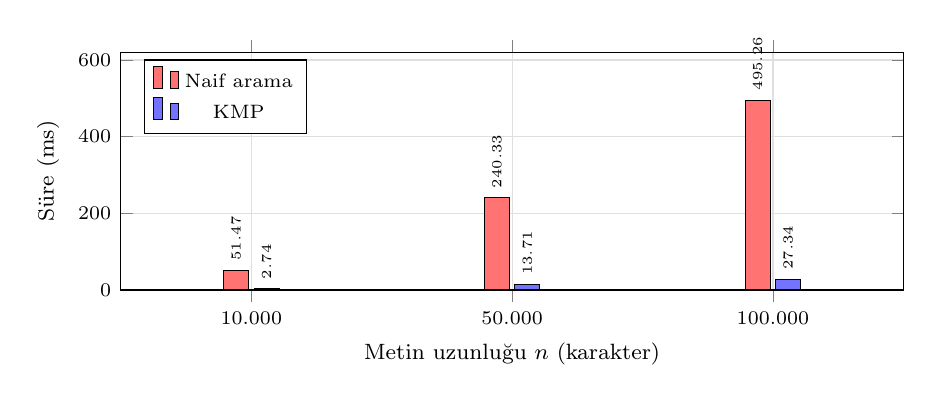
\begin{tikzpicture}
\begin{axis}[
  width=0.95\columnwidth, height=4.6cm,
  ybar, bar width=9pt, ymin=0,
  xlabel={Metin uzunluğu $n$ (karakter)}, ylabel={Süre (ms)},
  symbolic x coords={10.000,50.000,100.000}, xtick=data,
  legend style={font=\scriptsize, at={(0.03,0.97)}, anchor=north west},
  tick label style={font=\scriptsize}, label style={font=\footnotesize},
  nodes near coords, nodes near coords style={font=\tiny, rotate=90, anchor=west},
  enlarge x limits=0.25, ymax=620,
  grid=major, grid style={gray!25}]
\addplot[fill=red!55] coordinates {(10.000,51.47) (50.000,240.33) (100.000,495.26)};
\addplot[fill=blue!55] coordinates {(10.000,2.74) (50.000,13.71) (100.000,27.34)};
\legend{Naif arama, KMP}
\end{axis}
\end{tikzpicture}
\caption{En kötü durum girdisinde ($m=50$) naif arama ve KMP süreleri.}
\label{fig:kmp}
\end{figure}

\textit{3) Geri alma bellek kullanımı:} 1000 tek karakterlik düzenleme için işlem tabanlı yaklaşımın ve her düzenlemeden önce metnin kopyasını alan anlık görüntü yaklaşımının bellek kullanımları Tablo~\ref{tab:bellek} üzerinde karşılaştırılmıştır. İşlem tabanlı yaklaşımın bellek kullanımı dosya boyutundan bağımsız olarak yaklaşık 90 KB'dir. Anlık görüntü yöntemi ise 404,5 KB'lık bir dosya için yaklaşık 809 MB bellek gerektirmektedir; bu, yaklaşık 9000 katlık bir farktır.

\begin{table}[t]
\centering
\caption{1000 Düzenleme İçin Geri Alma Geçmişinin Bellek Kullanımı}
\label{tab:bellek}
\begin{tabular}{@{}rrrr@{}}
\toprule
\textbf{Dosya boyutu} & \textbf{İşlem kaydı} & \textbf{Anlık görüntü} & \textbf{Oran} \\
\midrule
8,0 KB & 90,0 KB & 16,11 MB & $\approx$179$\times$ \\
81,2 KB & 90,0 KB & 162,55 MB & $\approx$1806$\times$ \\
404,5 KB & 90,0 KB & 809,00 MB & $\approx$8989$\times$ \\
\bottomrule
\end{tabular}
\end{table}

\textit{4) Toplu değiştirme ve geri alma:} 1.000 satırlık bir metinde 918 eşleşme 18,2~ms'de değiştirilmiş ve tek bir \kod{Ctrl+Z} ile 2,2~ms'de geri alınmıştır. 10.000 satır ve 9.058 eşleşme için bu süreler sırasıyla 243,4~ms ve 38,1~ms'dir. Her iki durumda da geri alma sonrası metnin orijinal metinle karakter karakter aynı olduğu doğrulanmıştır.

\textit{5) Ekran çizimi ve ölçüme dayalı iyileştirme:} 120$\times$30 boyutlu bir pencerede bir ekran karesinin çizimi ölçülmüştür. İlk ölçümlerde, arama vurgusu açıkken çizim süresinin dosya boyutuyla birlikte hızla arttığı görülmüştür: 50.000 satırlık bir dosyada kare başına 108,85~ms. İncelendiğinde, her karede ekranda görünmeyenler dahil 45.596 eşleşmenin tamamının tarandığı tespit edilmiştir. Eşleşme listesi $(r,c)$ sırasına göre zaten sıralı olduğu için, yalnızca görünen satır aralığına düşen eşleşmeler ikili arama (\kod{bisect}) ile $O(\log k)$ sürede bulunacak şekilde kod değiştirilmiştir. Tablo~\ref{tab:cizim}'de görüldüğü gibi bu iyileştirmeyle çizim süresi dosya boyutundan bağımsız hâle gelmiş ve en büyük dosyada yaklaşık 340 kat azalmıştır. Bir karenin çizimi 0,3~ms civarında sürdüğünden, kullanıcı tuşa bastığında gecikme algılanmamaktadır.

\begin{table}[t]
\centering
\caption{Arama Vurgusu Açıkken Kare Başına Çizim Süresi (ms)}
\label{tab:cizim}
\begin{tabular}{@{}rrrr@{}}
\toprule
\textbf{Satır sayısı} & \textbf{Eşleşme} & \textbf{İyileştirme öncesi} & \textbf{Sonrası} \\
\midrule
100 & $\approx$90 & 0,31 & 0,34 \\
10.000 & $\approx$9.000 & 11,97 & 0,30 \\
50.000 & 45.596 & 108,85 & 0,32 \\
\bottomrule
\end{tabular}
\end{table}

\subsection{Karşılaşılan Sorunlar ve Çözümleri}

Geliştirme ve test sürecinde karşılaşılan başlıca sorunlar şunlardır:

\textit{1) Terminal öykünücülerinin kısayolları yakalaması:} Uygulama PyCharm geliştirme ortamının içinden çalıştırıldığında \kod{Ctrl+H} (Type Hierarchy) ve \kod{Ctrl+Backspace} gibi tuşların uygulamaya ulaşmadan geliştirme ortamı tarafından yakalandığı görülmüştür. Benzer şekilde Windows Terminal, \kod{Ctrl+Shift+Yukarı/Aşağı} tuşlarını kendi kaydırma işlemi için kullanmaktadır. Çözüm olarak uygulamanın klasik Windows konsolunda (\kod{conhost}) çalıştırılması belirlenmiştir.

\textit{2) Ctrl+H ve Backspace karışıklığı:} ASCII'de \kod{Ctrl+H} ile Backspace aynı koda sahip olduğu için bazı terminallerde \kod{Ctrl+H} Backspace olarak algılanmıştır. Sorun, tuş çözümleme sırasında tarama kodu ve karakter değeri kontrol edilerek giderilmiştir (Tablo~\ref{tab:tus}, kural~1).

\textit{3) AltGr karakterleri:} Türkçe klavyede \kod{@} ve \kod{\{} gibi karakterlerin ``Ctrl+Alt'' olarak raporlanması nedeniyle bu karakterlerin kısayol olarak yorumlanma riski, Ctrl ile Alt birlikte basılıyken olayın karakter sayılmasıyla önlenmiştir.

\textit{4) Çalıştırılabilir dosya üretimi:} Anaconda ortamında yüklü olan eski \kod{pathlib} geri taşıma (backport) paketinin PyInstaller ile uyumsuz olduğu görülmüş; paket kaldırılarak sorun çözülmüştür. Derleme betiği de hata durumunda başarılı mesajı vermeyecek şekilde düzeltilmiştir.

% ================================================================ SONUÇ
\section{Sonuç}\label{sec:sonuc}

Bu çalışmada proje tanımındaki tüm gereksinimleri karşılayan, konsol tabanlı ve yalnızca klavyeyle yönetilen bir metin editörü geliştirilmiştir. Python standart kütüphanesi ile Windows konsol API'sine doğrudan erişilerek, harici bir kütüphane kullanılmadan ham klavye girişi, renkli vurgulama ve özelleştirilmiş imleç elde edilmiştir. Veri yapısı ve algoritma tercihleri hem kuramsal olarak gerekçelendirilmiş hem de deneysel olarak doğrulanmıştır: satır listesi yapısı ekleme maliyetini dosya boyutundan bağımsız hâle getirmiş, KMP algoritması en kötü durumda naif aramadan yaklaşık 18 kat hızlı çalışmış, işlem tabanlı geri alma ise bellek kullanımını binlerce kat azaltmıştır. Ölçümler sırasında tespit edilen bir çizim darboğazı ikili arama ile giderilerek çizim süresi yaklaşık 340 kat iyileştirilmiştir. Bağımlılık enjeksiyonuna dayalı mimari sayesinde uygulamanın tamamı 36 uçtan uca senaryoyla otomatik olarak test edilebilmiştir.

Uygulamanın bazı sınırlamaları bulunmaktadır. Sekme karakterleri dört boşluğa dönüştürülmekte, ekrandaki her karakterin tek hücre genişliğinde olduğu varsayılmaktadır; bu nedenle emoji gibi çift genişlikli karakterler hizalamayı bozabilir. İleri alma (redo) desteği yoktur. Çok büyük dosyalarda (milyonlarca karakter) \kod{Ctrl+F} sırasında her tuşta yeniden yapılan arama yarım saniyeye ulaşabilmektedir. Platform katmanı yalnızca Windows için yazılmıştır.

Gelecek çalışmalarda ikinci bir yığın ile ileri alma desteğinin eklenmesi, çok büyük dosyalar için piece table veya rope yapısına geçilmesi, aramanın yalnızca değişen satırlarda tekrarlanması, Boyer-Moore gibi alt-doğrusal ortalama süreli algoritmaların ve düzenli ifadelerin (regex) desteklenmesi, sözdizimi renklendirmesi ve Linux/macOS desteği için POSIX \kod{termios} tabanlı ikinci bir platform katmanı yazılması planlanmaktadır. Katmanlı mimari sayesinde son madde, üst katmanlarda değişiklik gerektirmeden yapılabilecektir.

% ================================================================ KAYNAKÇA
\begin{thebibliography}{99}

\bibitem{kmp}
D.~E. Knuth, J.~H. Morris, and V.~R. Pratt, ``Fast pattern matching in strings,'' \textit{SIAM Journal on Computing}, vol.~6, no.~2, pp.~323--350, 1977.

\bibitem{clrs}
T.~H. Cormen, C.~E. Leiserson, R.~L. Rivest, and C.~Stein, \textit{Introduction to Algorithms}, 3rd~ed. Cambridge, MA, USA: MIT Press, 2009.

\bibitem{finseth}
C.~A. Finseth, \textit{The Craft of Text Editing: Emacs for the Modern World}. New York, NY, USA: Springer-Verlag, 1991.

\bibitem{crowley}
C.~Crowley, ``Data structures for text sequences,'' Computer Science Department, University of New Mexico, Tech. Rep., 1998.

\bibitem{gof}
E.~Gamma, R.~Helm, R.~Johnson, and J.~Vlissides, \textit{Design Patterns: Elements of Reusable Object-Oriented Software}. Reading, MA, USA: Addison-Wesley, 1994.

\bibitem{ecma48}
ECMA International, ``Control functions for coded character sets,'' Standard ECMA-48, 5th~ed., 1991.

\bibitem{msvt}
Microsoft, ``Console virtual terminal sequences,'' \textit{Microsoft Learn}. [Online]. Available: \url{https://learn.microsoft.com/en-us/windows/console/console-virtual-terminal-sequences}

\bibitem{msinput}
Microsoft, ``ReadConsoleInput function,'' \textit{Microsoft Learn}. [Online]. Available: \url{https://learn.microsoft.com/en-us/windows/console/readconsoleinput}

\bibitem{msmode}
Microsoft, ``SetConsoleMode function,'' \textit{Microsoft Learn}. [Online]. Available: \url{https://learn.microsoft.com/en-us/windows/console/setconsolemode}

\bibitem{pyctypes}
Python Software Foundation, ``ctypes --- A foreign function library for Python,'' \textit{Python 3 Documentation}. [Online]. Available: \url{https://docs.python.org/3/library/ctypes.html}

\bibitem{pyinstaller}
PyInstaller Development Team, ``PyInstaller manual.'' [Online]. Available: \url{https://pyinstaller.org/en/stable/}

\bibitem{npp}
D.~Ho, ``Notepad++: A free source code editor.'' [Online]. Available: \url{https://notepad-plus-plus.org/}

\end{thebibliography}

\end{document}
